\documentclass{article}
\usepackage{siunitx}
%% Language and font encodings
\usepackage[english]{babel}
\usepackage[utf8x]{inputenc}
\usepackage[T1]{fontenc}
\usepackage{longtable}
\usepackage{multirow}

%% Sets page size and margins
\usepackage[a4paper,top=3cm,bottom=2cm,left=3cm,right=3cm,marginparwidth=1.75cm]{geometry}

%% Useful packages
\usepackage{amsmath}
\usepackage{graphicx,float}
\usepackage[colorinlistoftodos]{todonotes}
\usepackage[colorlinks=true, allcolors=blue]{hyperref}

\title{CSP334: Computer Networks \linebreak
Lab Assignment No 1 \linebreak
Assignment on Linux Networking Commands}
\author{Abhishek Gupta  2016UCS0012}

\begin{document}
\maketitle

\section{Q1: Network Interfaces}
 \begin{figure}[H]
 \centering
 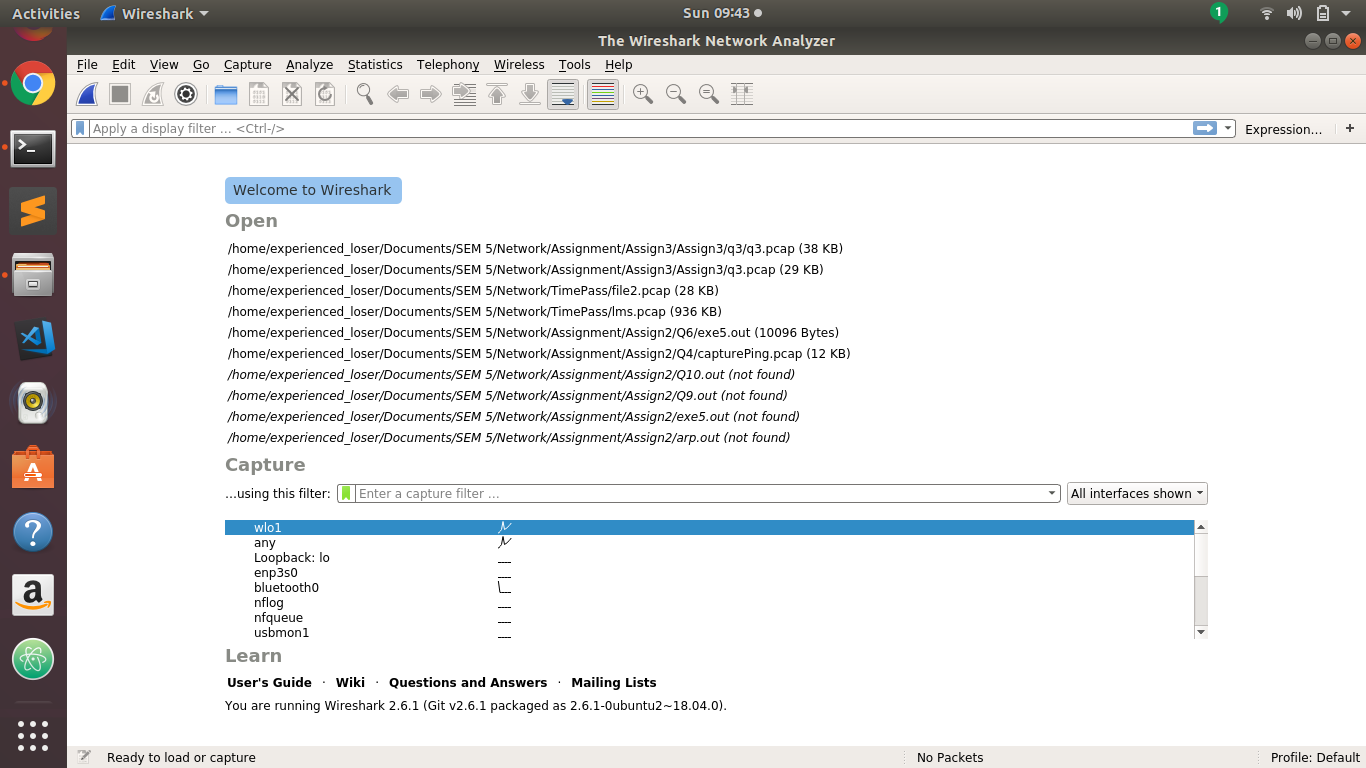
\includegraphics[width=1.0\textwidth]{../q1/a.png}
 \caption{\label{fig:PING}Screenshot of Network Interfaces}
 \end{figure}
 
 I selected \textbf{wlo1} network interface
 
 
\section{Q2: Application Layer Protocol}

\textbf{HTTP} Application Protocol is used
 
\section{Q3: Protocols Displayed in Unfiltered Packet}

The following protocols were displaced in Unfiltered Packet :-
\begin{enumerate}
	\item ARP
	\item DNS
	\item TCP
	\item TLSv1.2
\end{enumerate}
 
\section{Q4: IPA}
 \begin{figure}[H]
 \centering
 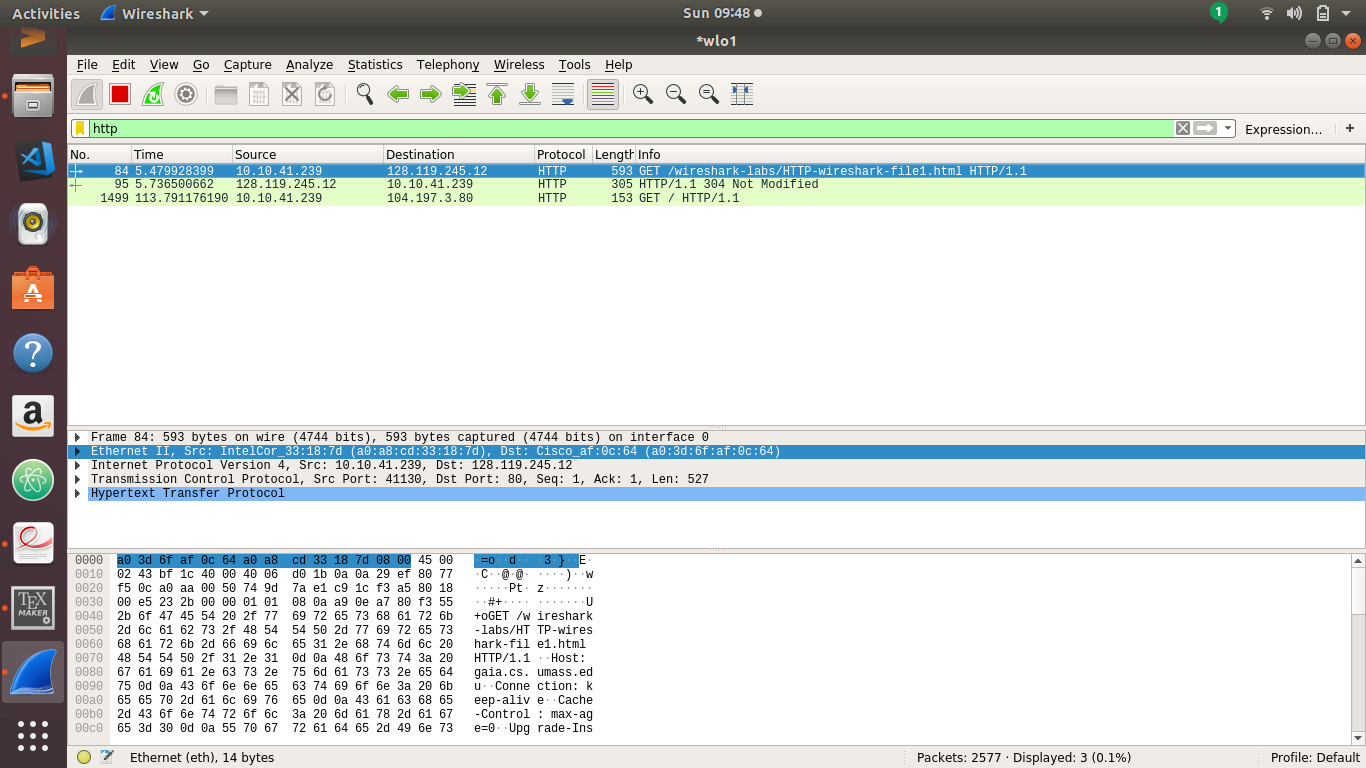
\includegraphics[width=1.0\textwidth]{../q4/a.png}
 \caption{\label{fig:PING}Screenshot of IPA}
 \end{figure}
 
IPA of my machine          : \textbf{10.10.41.239} \\
IPA of destination machine : \textbf{128.119.245.12}

\subsection{How did I confirm destination IP}
I did nslookup of http://gaia.cs.umass.edu/wireshark-labs/HTTP-wireshark-file1.html and got :
 \begin{figure}[H]
 \centering
 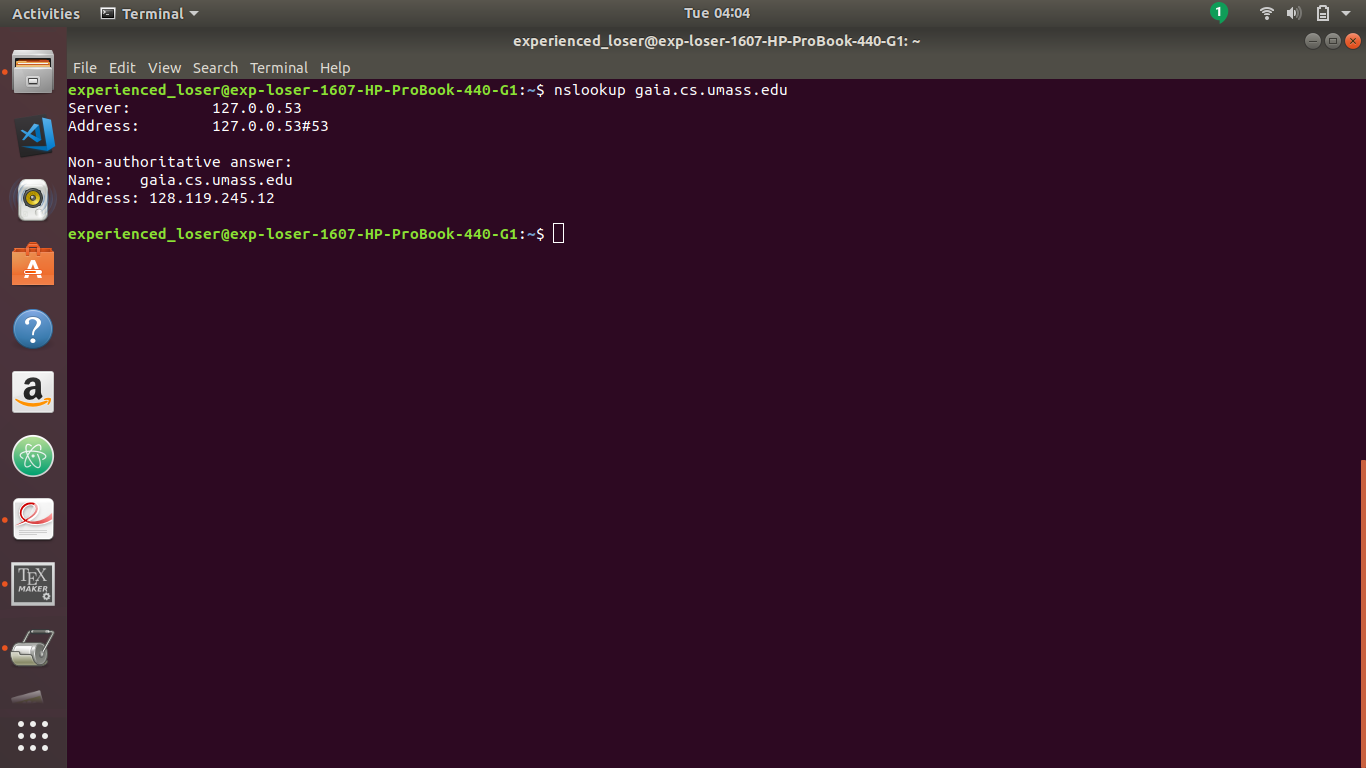
\includegraphics[width=1.0\textwidth]{../q4/b.png}
 \caption{\label{fig:PING}Screenshot of dest IP}
 \end{figure}
 
 \textbf{Hence IPA of Dest Verified}
 
\section{Q5: Class of IPA}
 source      : \textbf{CLASS A}\\
 destination : \textbf{CLASS B}
 
 
\section{Q6: Bits captured}
 \begin{figure}[H]
 \centering
 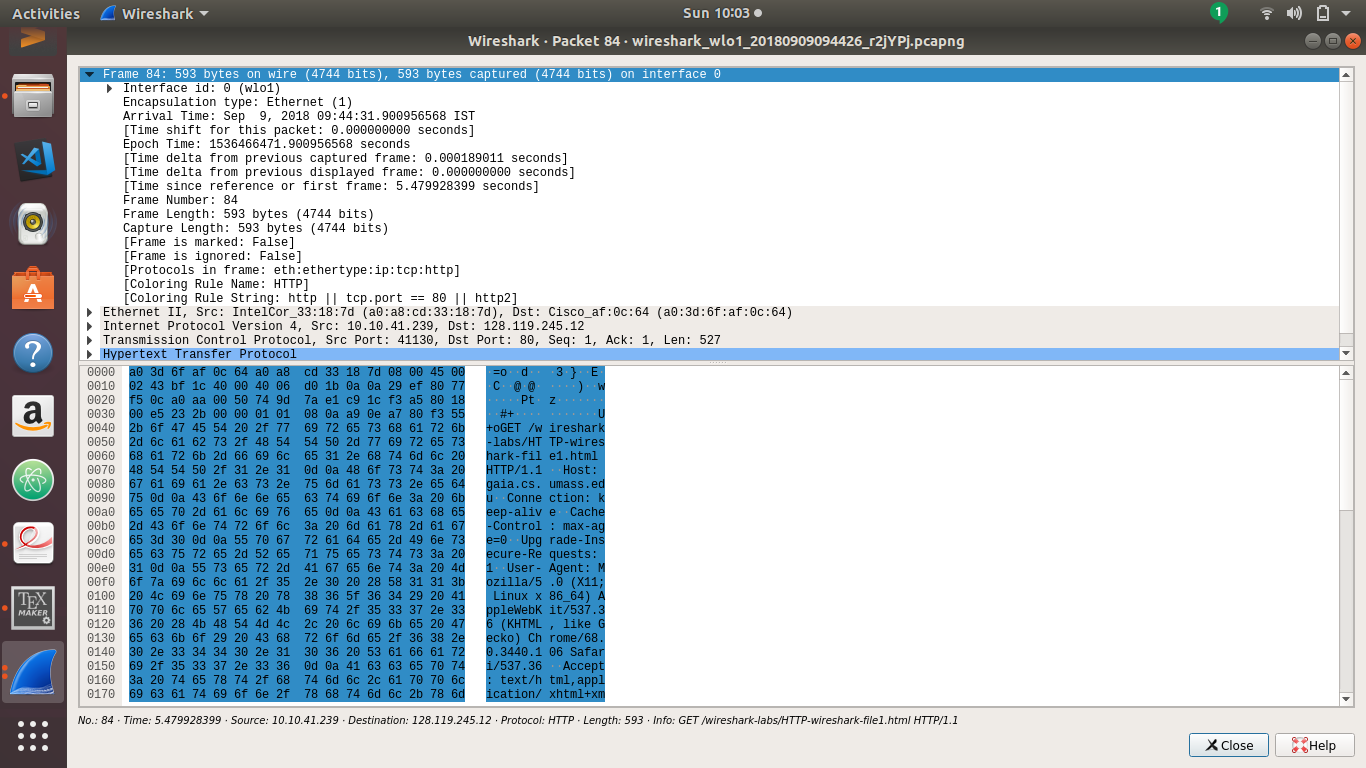
\includegraphics[width=1.0\textwidth]{../q6/a.png}
 \caption{\label{fig:PING}Screenshot of captured Bits}
 \end{figure}
 
 593 Bytes ie 593 X 8 = \textbf{4744} Bits were captured on \textbf{ Sep 9 2018 at 9:44:31 IST}
 
\section{Q7: Interface id}
 \begin{figure}[H]
 \centering
 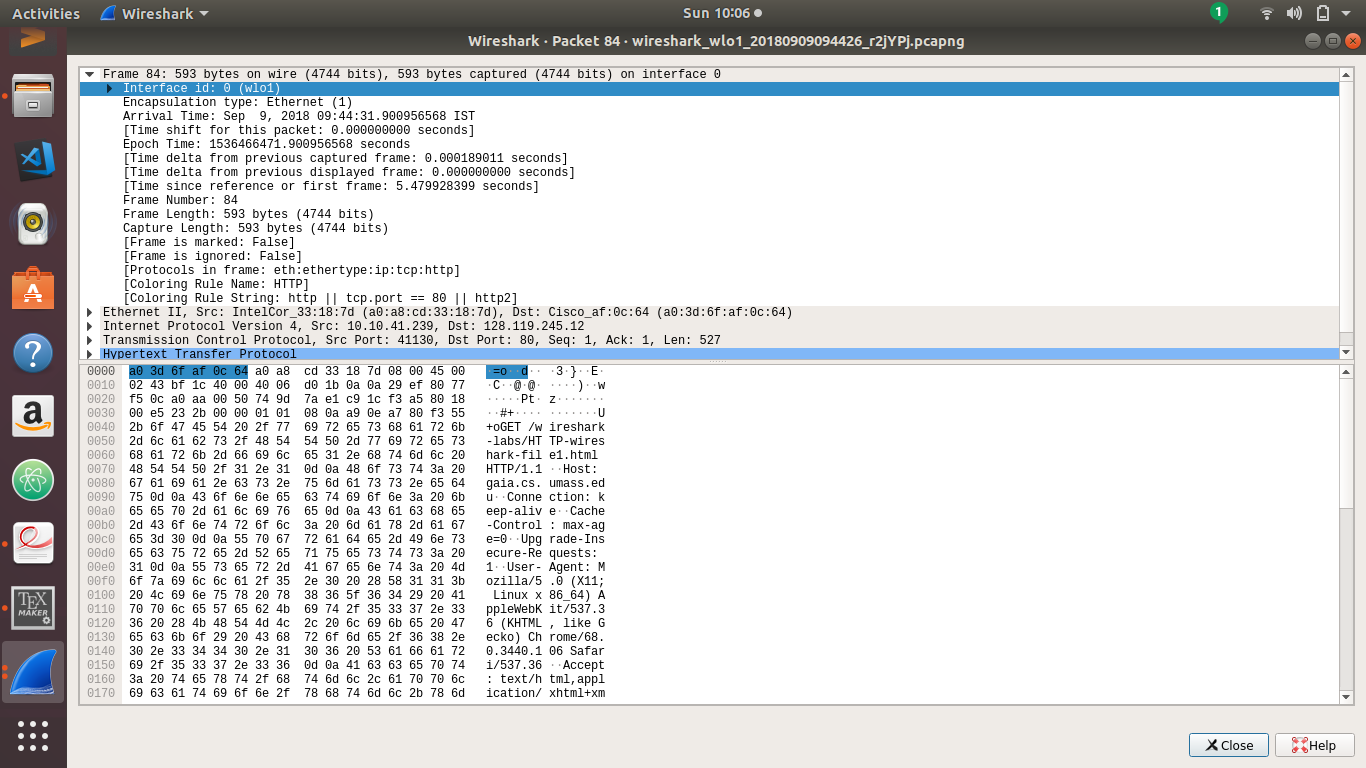
\includegraphics[width=1.0\textwidth]{../q7/a.png}
 \caption{\label{fig:PING}Screenshot of interface id}
 \end{figure}
 
 Interface Id     : 0\\
 Interface Address: wlo1\\
 
 
\section{Q8: Time for HTTP OK reply to Receive}
 \begin{figure}[H]
 \centering
 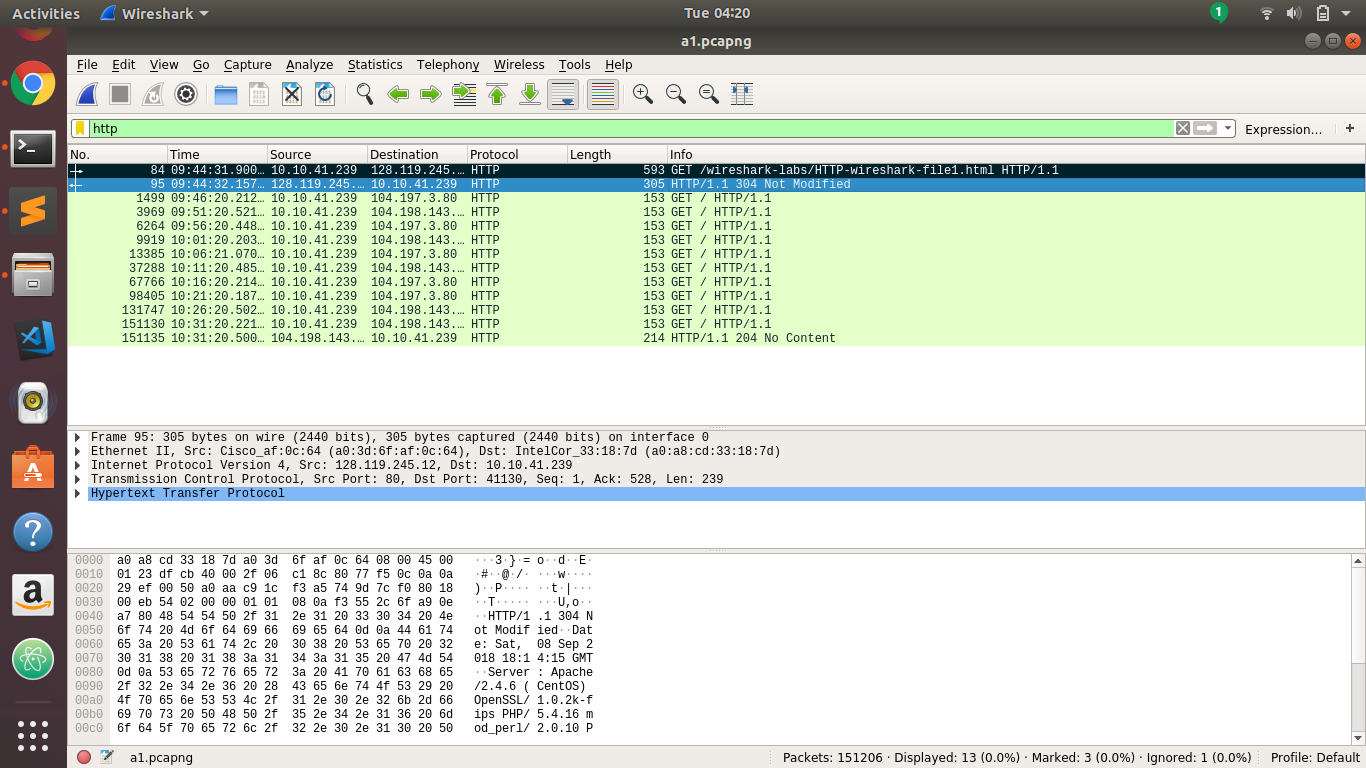
\includegraphics[width=1.0\textwidth]{../q8/a.png}
 \caption{\label{fig:PING}Screenshot of http filtered packets}
 \end{figure}
  
  
 Request (Black Highlighted) at \textbf{9:44:31:900 IST}\\
 Response (Blue Highlighted) at \textbf{9:44:32.157 IST}\\
 
 Site took \textbf{0.257 sec} to respond\\
 
\section{Q9 : No such question}

\section{Q10: 2 HTTP messages}
 \begin{figure}[H]
 \centering
 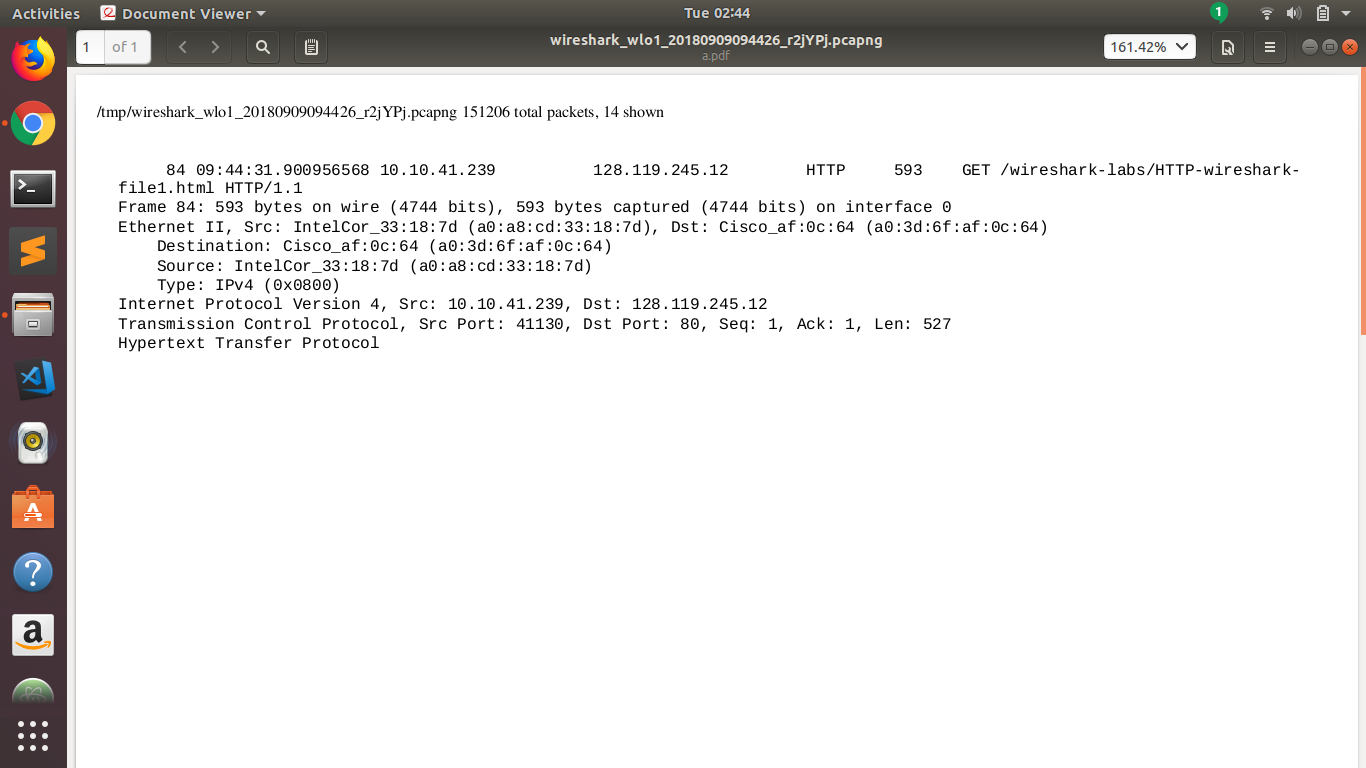
\includegraphics[width=1.0\textwidth]{../q10/a.png}
 \caption{\label{fig:PING}Screenshot of http message 1}
 \end{figure}
 
  \begin{figure}[H]
 \centering
 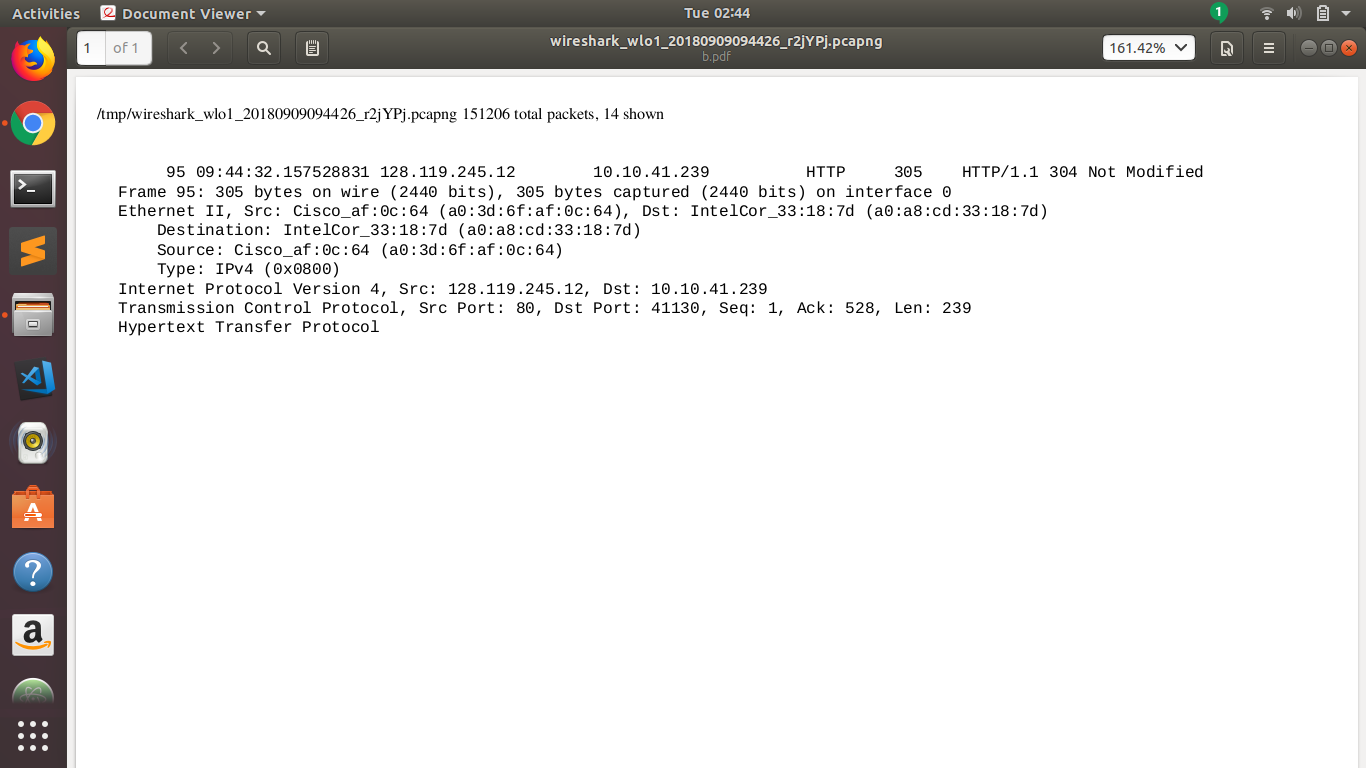
\includegraphics[width=1.0\textwidth]{../q10/b.png}
 \caption{\label{fig:PING}Screenshot of http message 2}
 \end{figure}
 
\section{Q11: Destination Physical Address}
 \begin{figure}[H]
 \centering
 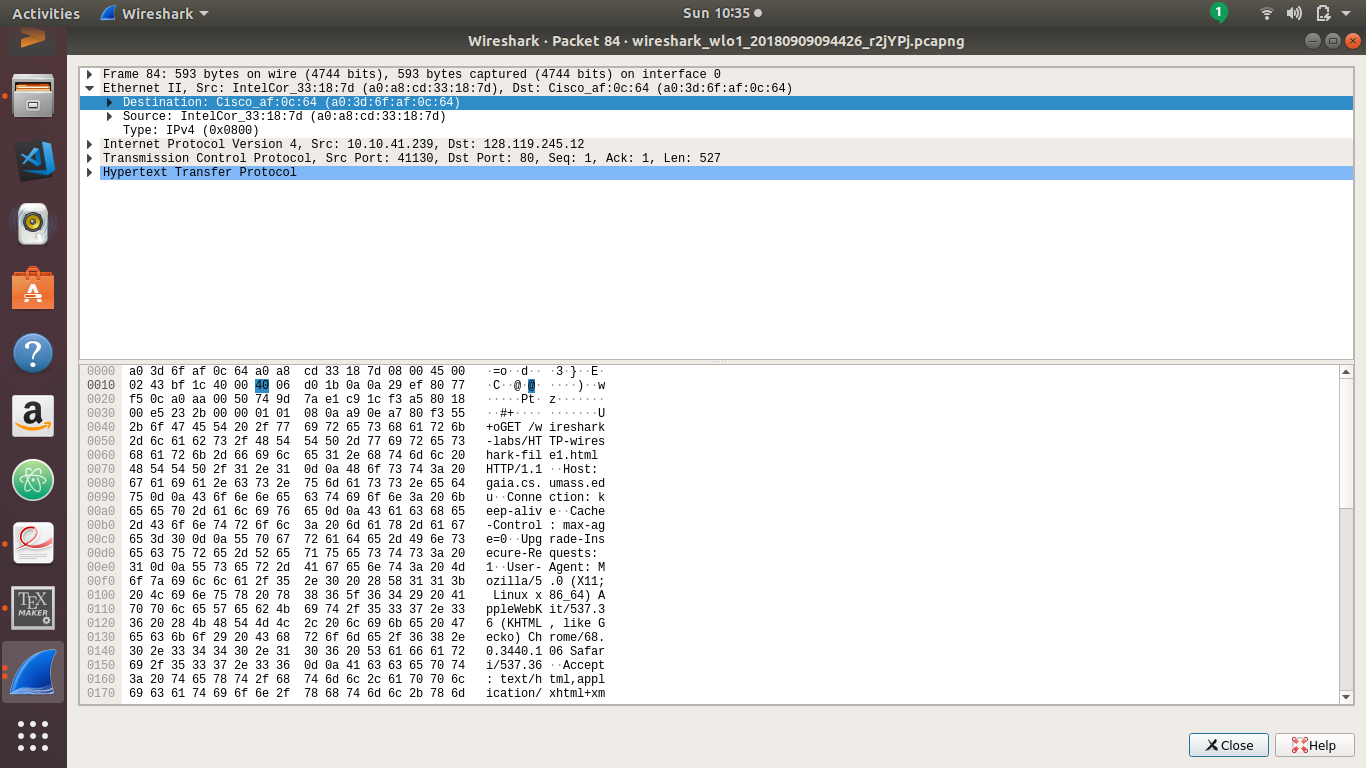
\includegraphics[width=1.0\textwidth]{../q11/a.png}
 \caption{\label{fig:PING}Screenshot of dest physical address}
 \end{figure}
 
 Destination Physical Address : \textbf{$Cisco_af:0c:64 (a0:3d:6f:af:0c:64)$}\\
 This belong to the physical address of our gateway ie the first router of our system\\
 
 
\section{Q12: Length of header}
 \begin{figure}[H]
 \centering
 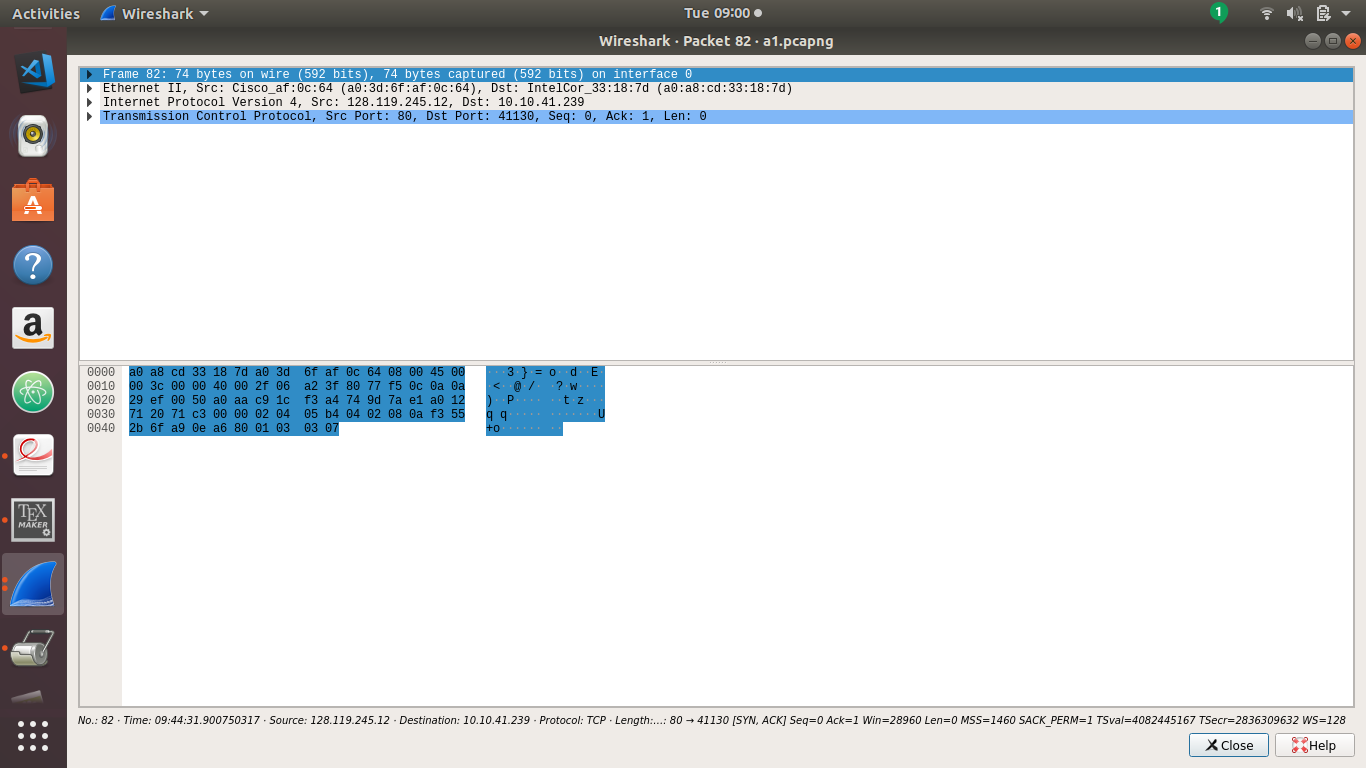
\includegraphics[width=1.0\textwidth]{../q12/a.png}
 \caption{\label{fig:PING}Screenshot of tcp header}
 \end{figure}
 

Total \textbf{74 Byte}
 
\section{Q13: Ethernet header of a frame}
 \begin{figure}[H]
 \centering
 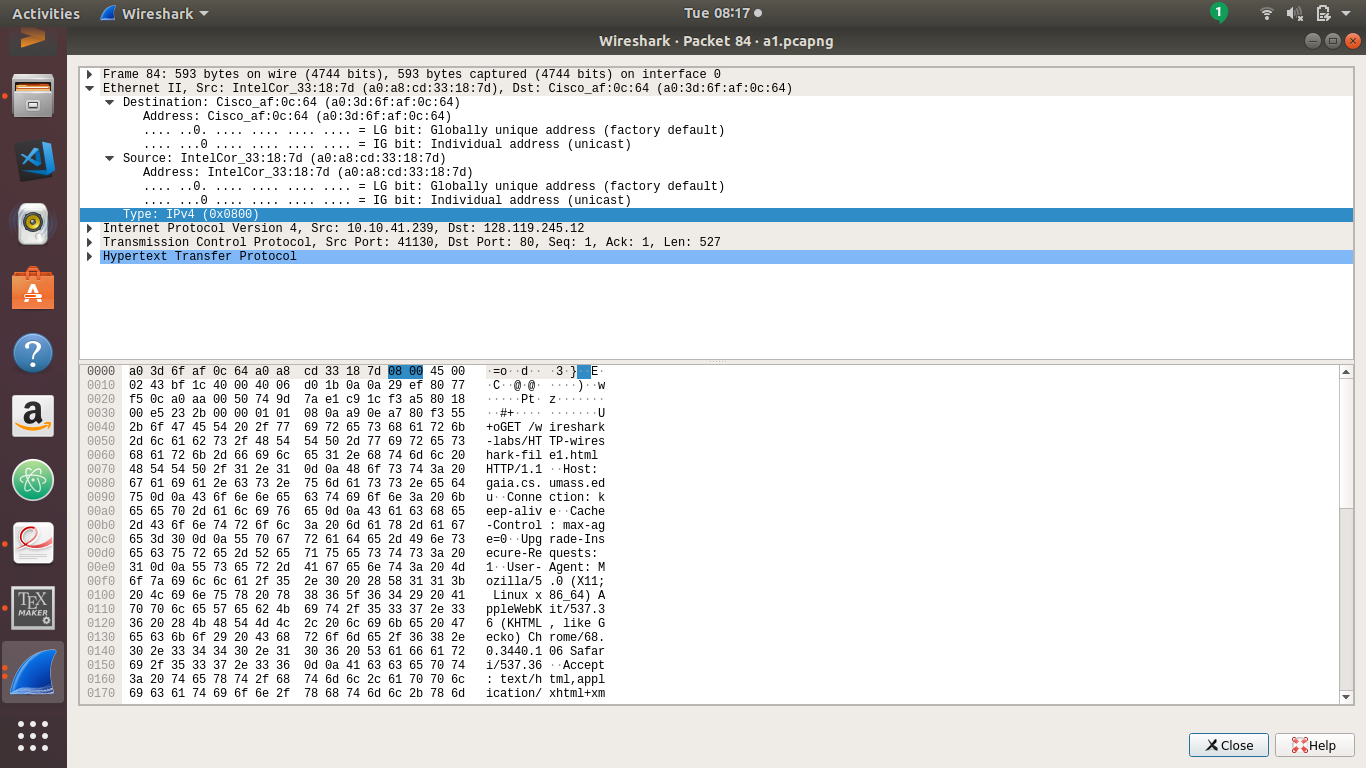
\includegraphics[width=1.0\textwidth]{../q13/a.png}
 \caption{\label{fig:PING}Screenshot of ethernet header frame}
 \end{figure}
 
 Yes we can determine and above is the proof.
 
 
\section{Q14: TCP or UDP as transport protocol}
 \begin{figure}[H]
 \centering
 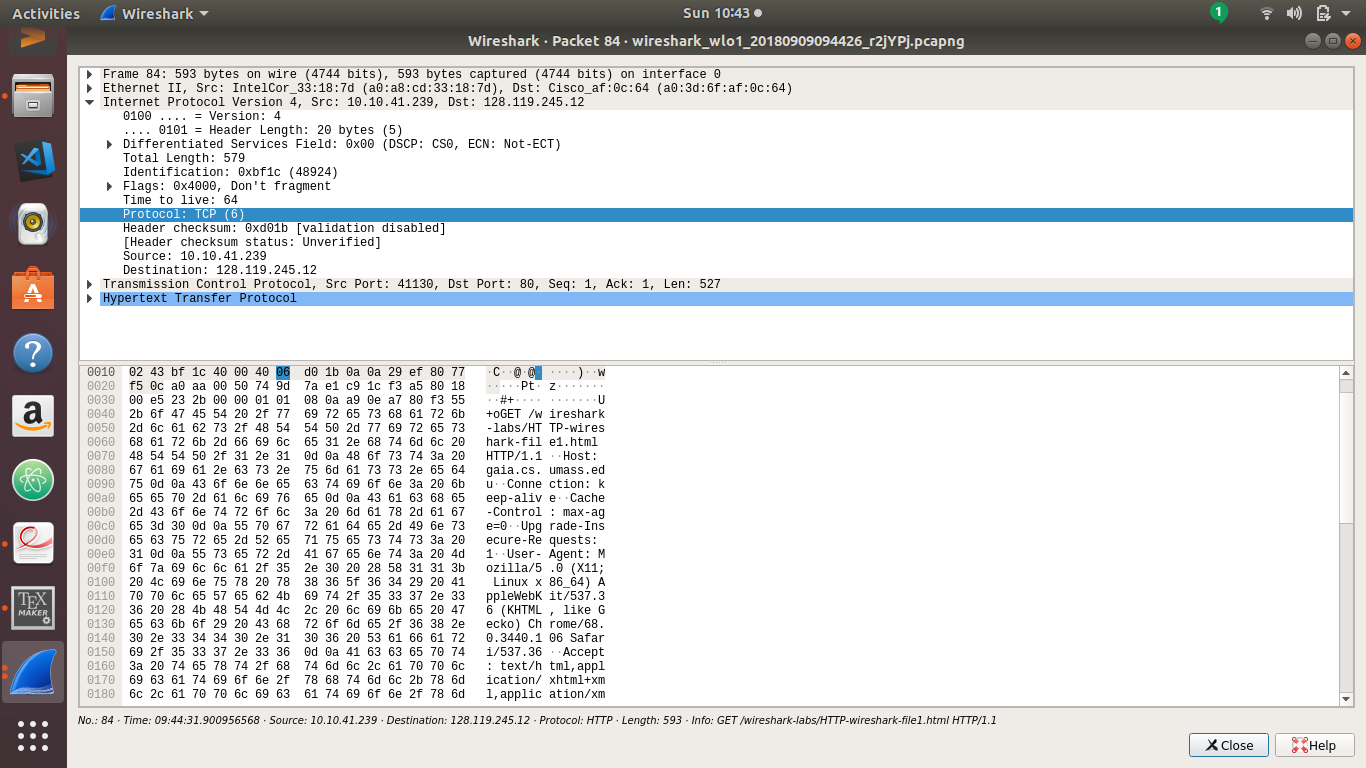
\includegraphics[width=1.0\textwidth]{../q14/a.png}
 \caption{\label{fig:PING}Screenshot of tcpdump file}
 \end{figure}
Yes it is possible to know whether the first packet captured has TCP or UDP as transport protocol . The upper picture is the proof. Highlighted TCP(6)\\
 
\section{Q15: SYN and ACK}
 \begin{figure}[H]
 \centering
 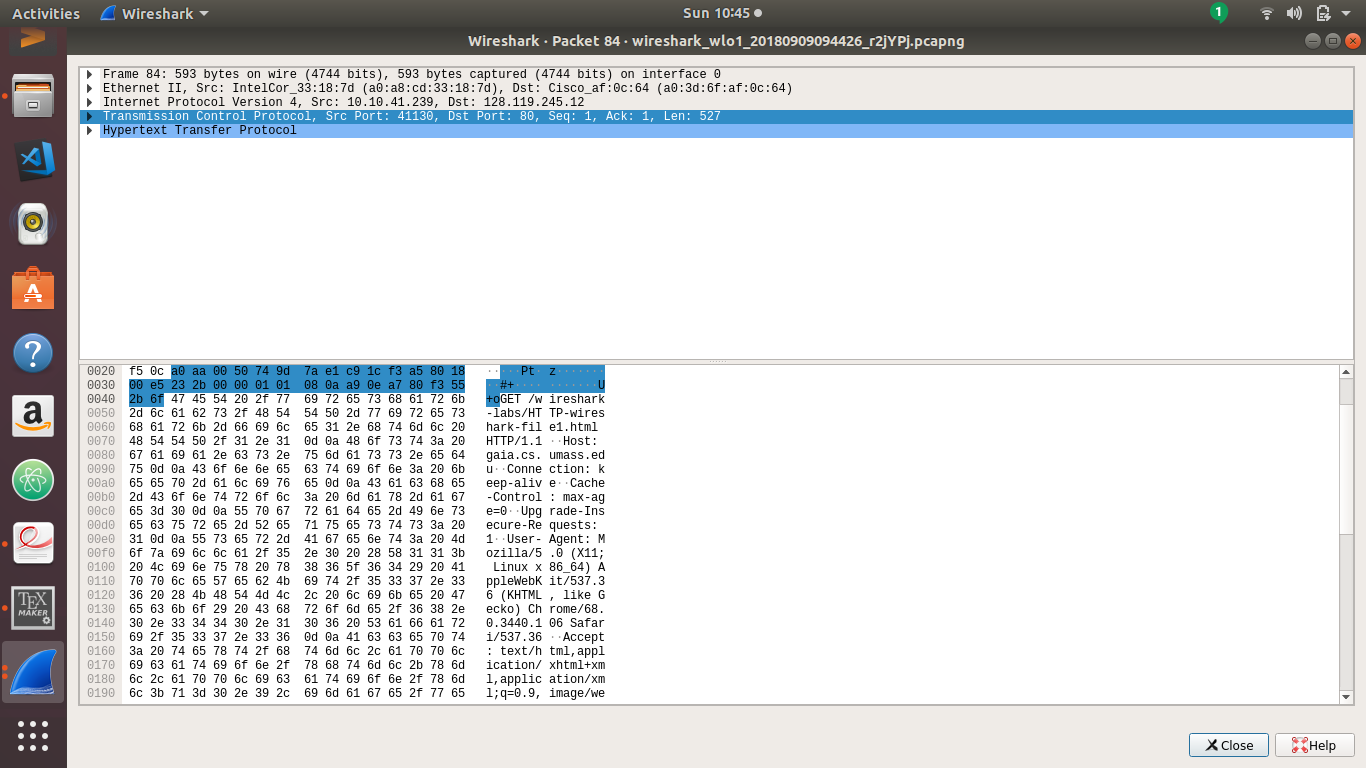
\includegraphics[width=1.0\textwidth]{../q15/a.png}
 \caption{\label{fig:PING}Screenshot of request from client}
 \end{figure}
 
 Ports (SYN) request from client:\\ \\
 \\
 Client Port: 41139 \\
 Server Port: 80 \\
 
  \begin{figure}[H]
 \centering
 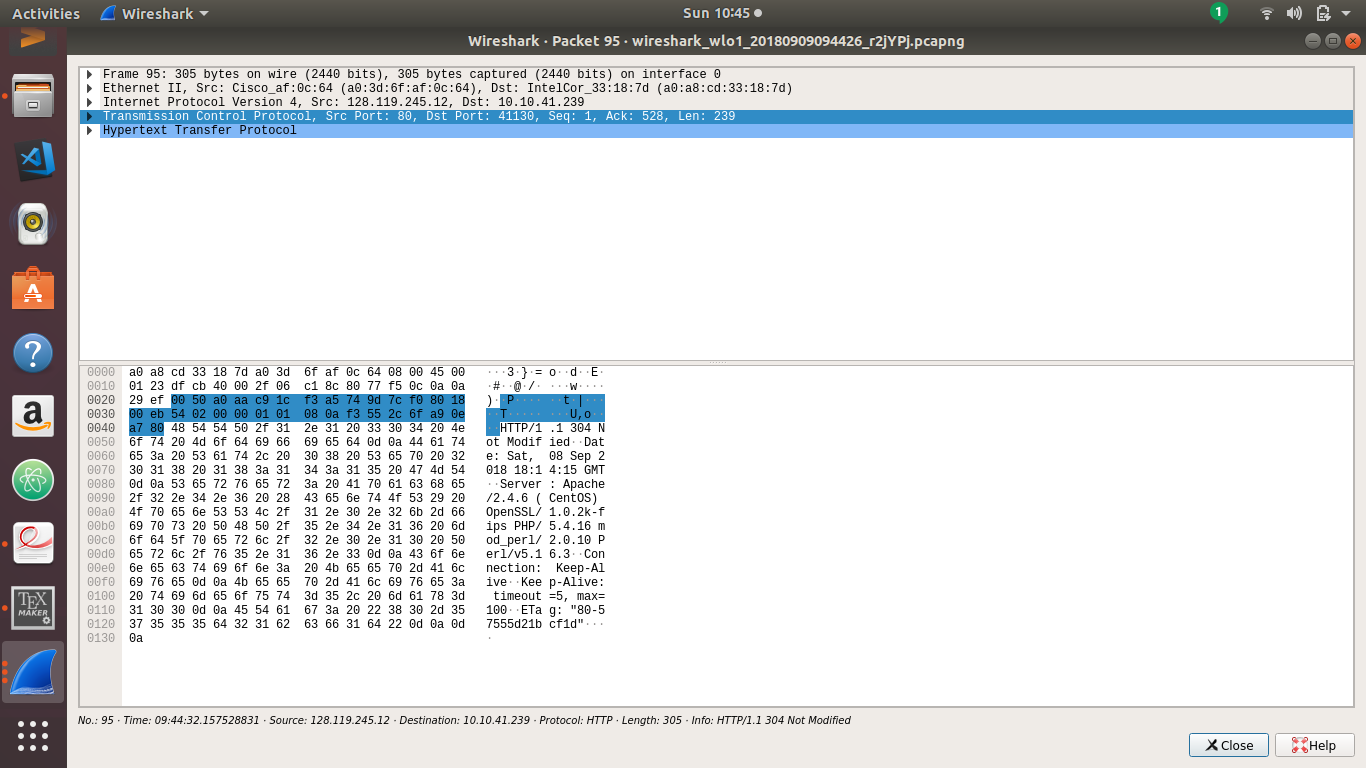
\includegraphics[width=1.0\textwidth]{../q15/b.png}
 \caption{\label{fig:PING}Screenshot of response from server}
 \end{figure}
 
  Ports (ACK) response from server:\\ \\
 \\
 Client Port: 41139 \\
 Server Port: 80 \\
 
 \textbf{We can see that the client and server Port is \textbf{NOT} Same as thw one is well known port and other is empheral port which can change for many requests}
 
\section{Q16: Server Hello Message}
  \begin{figure}[H]
 \centering
 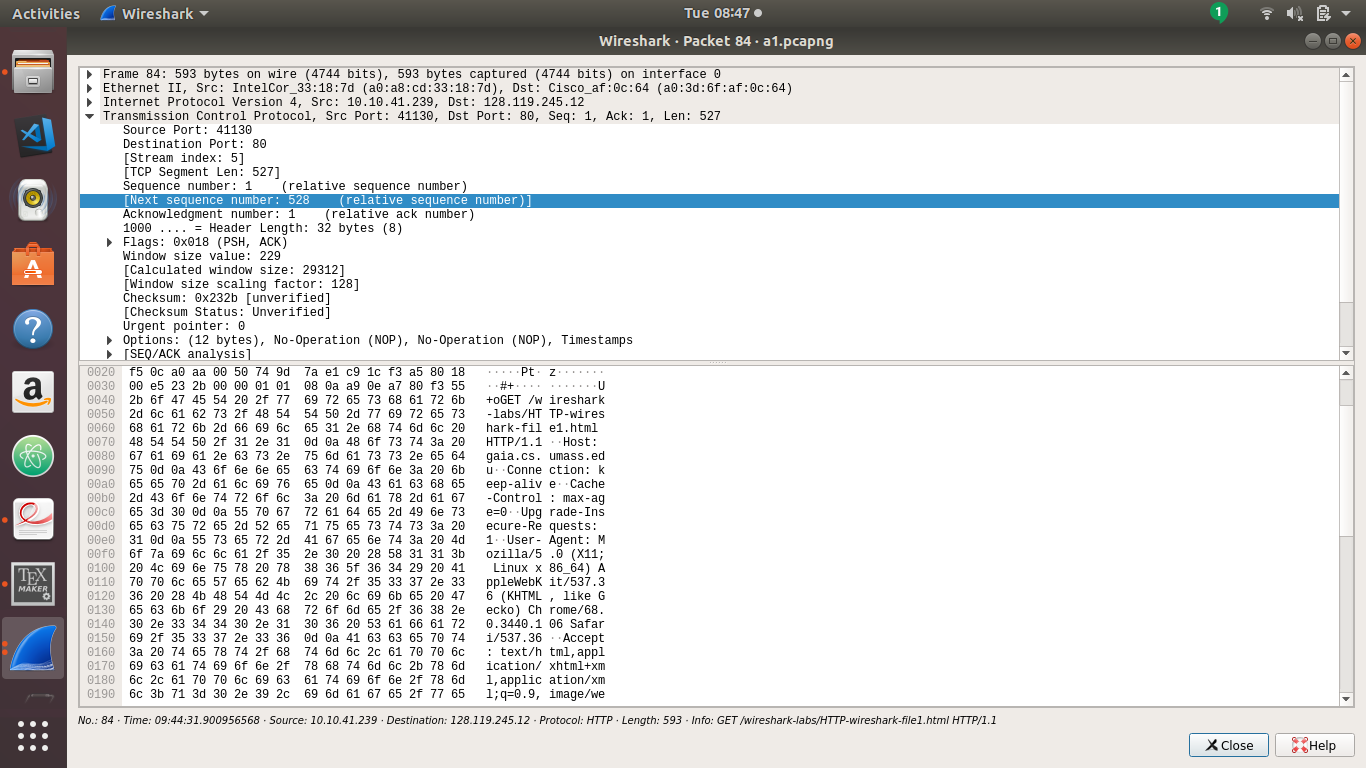
\includegraphics[width=1.0\textwidth]{../q16/a.png}
 \caption{\label{fig:PING}Screenshot of request}
 \end{figure}
 
 We can see that the next sequence number in the image is 528. Which will become ACK for the server.
 
 \begin{figure}[H]
 \centering
 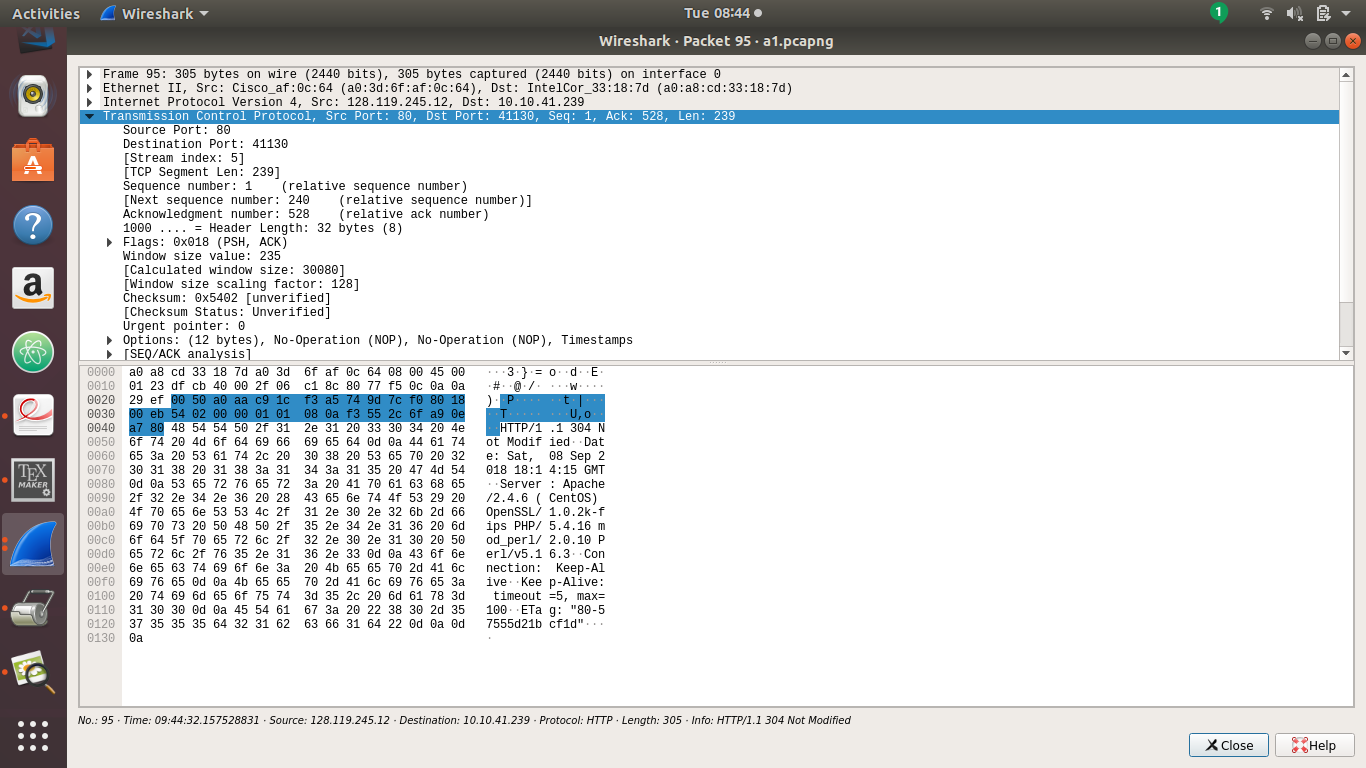
\includegraphics[width=1.0\textwidth]{../q16/b.png}
 \caption{\label{fig:PING}Screenshot of response}
 \end{figure}
Server Hello message sent by the server have 1 as a relative sequence number
and 528 as a relative acknowledgement number not 185.\\

Becoz of 3-way-handshake the next sequence number in the request packet becomes ACK number in the response packet. Now the ACK from client would be 240 in next request packet.
 
\section{Q17: First Sequence number sent by the server to the client}
 \begin{figure}[H]
 \centering
 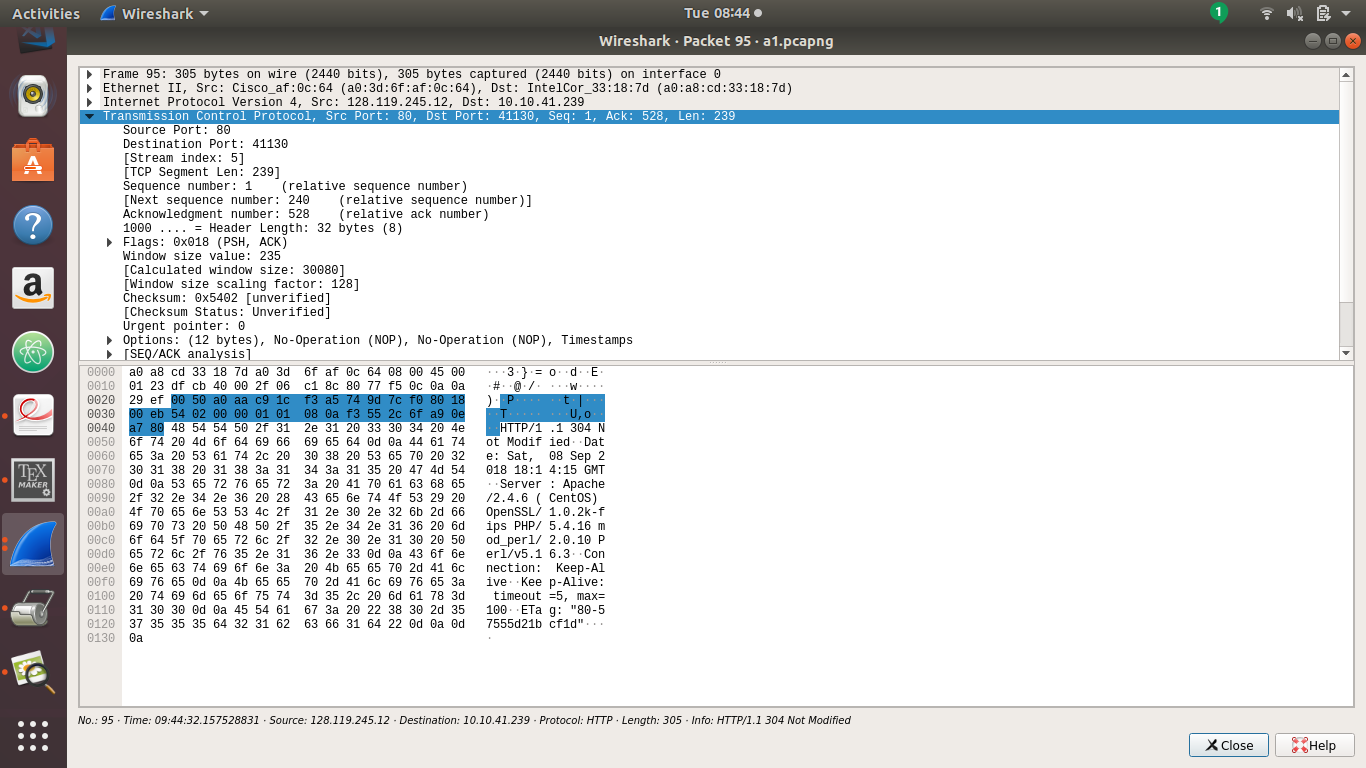
\includegraphics[width=1.0\textwidth]{../q16/b.png}
 \caption{\label{fig:PING}Screenshot of response}
 \end{figure}
 
 the first sequence number sent by the server to the client is 1.\\
 
 Let’s see what happens if sequence number is initiated as ‘0’ ,\\
 
  \begin{figure}[H]
 \centering
 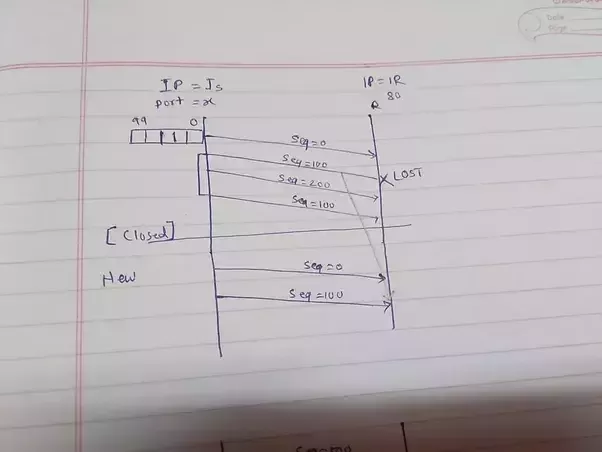
\includegraphics[width=1.0\textwidth]{../q17/a.png}
 \caption{\label{fig:PING}Screenshot of explanation}
 \end{figure}
 
 A sender sends 100B segment with initial sequence number as zero then next with sequence number 100 and so on. Consider that seq no 100 segment was delayed or lost and all three(assume only three) segments are transferred as well as that TCP connection was closed. Now a new connection with same IP:port as previous connection is established again and sequence number is initialized to ‘0’. now that delayed sequence number 100 seg is arrived now at seq num 100 of new connection as shown in picture, now that’s an issue here.

\end{document}